\documentclass[aspectratio=169,11pt]{beamer}
\usepackage{fontspec,xeCJK}
\setmainfont{texgyreheros-regular.otf}[BoldFont=texgyreheros-bold.otf,ItalicFont=texgyreheros-italic.otf]
\setsansfont{texgyreheros-regular.otf}[BoldFont=texgyreheros-bold.otf,ItalicFont=texgyreheros-italic.otf]
\setCJKmainfont{HaranoAjiGothic-Regular.otf}[BoldFont=HaranoAjiGothic-Bold.otf]
\setCJKsansfont{HaranoAjiGothic-Regular.otf}[BoldFont=HaranoAjiGothic-Bold.otf]
\usepackage{amsmath,amssymb,booktabs,array,tikz}
\usetikzlibrary{arrows.meta,patterns,decorations.markings}
\definecolor{ink}{HTML}{17324D}
\definecolor{accent}{HTML}{157C85}
\definecolor{light}{HTML}{EFF5F6}
\definecolor{muted}{HTML}{536575}
\setbeamercolor{normal text}{fg=ink,bg=white}
\setbeamercolor{frametitle}{fg=ink,bg=white}
\setbeamercolor{structure}{fg=accent}
\setbeamercolor{block title}{fg=white,bg=accent}
\setbeamercolor{block body}{fg=ink,bg=light}
\setbeamerfont{frametitle}{size=\Large,series=\bfseries}
\setbeamersize{text margin left=8mm,text margin right=8mm}
\setbeamertemplate{navigation symbols}{}
\setbeamertemplate{frametitle}{\vspace{2mm}\insertframetitle\par\vspace{1.5mm}{\color{accent}\hrule height .6pt}}
\setbeamertemplate{footline}{\hspace{8mm}\color{muted}\fontsize{6}{7}\selectfont Zenstudy\quad 熱力学\hfill\insertframenumber\hspace{8mm}\vspace{2mm}}
\setlength{\parskip}{3pt}
\newcommand{\tagline}[1]{{\small\color{accent}\textbf{#1}}\par\vspace{1mm}}
\newcommand{\ask}[2]{\par\vspace{2mm}\textcolor{accent}{\textbf{(#1)}}\quad #2\par}
\newcommand{\baseeq}{pV=nRT,\qquad U=\frac32nRT,\qquad Q=\Delta U+W}
\newcommand{\cyclefig}{%
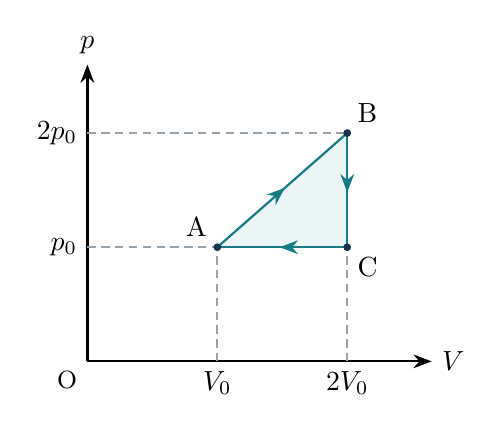
\begin{tikzpicture}[x=1.65cm,y=1.45cm,>=Stealth,line width=.8pt]
\fill[accent!8] (1,1)--(2,2)--(2,1)--cycle;
\draw[->] (0,0)--(2.65,0) node[right]{$V$};
\draw[->] (0,0)--(0,2.6) node[above]{$p$};
\node[below left] at (0,0) {\small O};
\draw[densely dashed,muted!60] (0,1)--(1,1) (0,2)--(2,2) (1,0)--(1,1) (2,0)--(2,1);
\node[left] at (0,1) {$p_0$}; \node[left] at (0,2) {$2p_0$};
\node[below] at (1,0) {$V_0$}; \node[below] at (2,0) {$2V_0$};
\draw[accent,thick,postaction={decorate},decoration={markings,mark=at position .52 with {\arrow{Stealth}}}] (1,1)--(2,2);
\draw[accent,thick,postaction={decorate},decoration={markings,mark=at position .52 with {\arrow{Stealth}}}] (2,2)--(2,1);
\draw[accent,thick,postaction={decorate},decoration={markings,mark=at position .52 with {\arrow{Stealth}}}] (2,1)--(1,1);
\foreach \x/\y in {1/1,2/2,2/1}{\fill[ink] (\x,\y) circle(1.4pt);}
\node[above left] at (1,1) {A}; \node[above right] at (2,2) {B}; \node[below right] at (2,1) {C};
\end{tikzpicture}}
\newcommand{\pistonfig}{%
\begin{tikzpicture}[x=.82cm,y=.82cm,>=Stealth,line width=.8pt]
\fill[accent!8] (.25,.25) rectangle(3.3,2.55);
\fill[pattern=north east lines,pattern color=muted!50] (0,0) rectangle(.25,2.8);
\fill[pattern=north east lines,pattern color=muted!50] (0,2.55) rectangle(4.8,2.8);
\fill[pattern=north east lines,pattern color=muted!50] (0,0) rectangle(4.8,.25);
\draw[thick] (4.8,0)--(0,0)--(0,2.8)--(4.8,2.8);
\draw[thick] (4.8,.25)--(.25,.25)--(.25,2.55)--(4.8,2.55);
\filldraw[fill=muted!25,thick] (3.3,.25) rectangle(3.58,2.55);
\draw[very thick,<-] (3.58,1.4)--(5.4,1.4) node[right]{$F$};
\node at (1.7,1.65) {理想気体};
\node at (1.7,1.05) {$p,\ V,\ T$};
\node[font=\small] at (4.45,2.1) {真空};
\draw[fill=white,line width=1.4pt,accent] (1.05,.08)--(2.1,.08);
\draw[accent,->] (1.55,-.65)--(1.55,.0);
\node[below,font=\small] at (1.55,-.65) {熱窓（開閉式）};
\draw[muted] (3.45,2.58)--(3.45,3.15);
\node[above,font=\small] at (3.45,3.15) {ピストン・断面積 $S$};
\end{tikzpicture}}

\hypersetup{pdftitle={熱力学 基本演習4題 解答・解説},pdfauthor={Zenstudy 教材制作}}
\begin{document}
\begin{frame}[t]{1\quad 三角形のサイクル\quad 〔温度・仕事〕}
\tagline{$pV$ から温度、グラフの面積から仕事を求める}
\begin{columns}[T,onlytextwidth]
\begin{column}{.59\textwidth}\small
\textbf{(1) 各状態の温度}\par
$pV=nRT$ より $T\propto pV$。したがって
\[\boxed{T_{\mathrm B}=4T_0},\qquad\boxed{T_{\mathrm C}=2T_0}.\]
\textbf{(2) 気体がする仕事}\par
AB は台形の面積、CA は圧縮なので負。
\begin{align*}
W_{\mathrm{AB}}&=\frac{p_0+2p_0}{2}(2V_0-V_0)=\boxed{\frac32p_0V_0},\\
W_{\mathrm{BC}}&=\boxed{0},\\
W_{\mathrm{CA}}&=p_0(V_0-2V_0)=\boxed{-p_0V_0}.
\end{align*}
\end{column}
\begin{column}{.37\textwidth}\centering\resizebox{\linewidth}{!}{\cyclefig}\end{column}
\end{columns}
\end{frame}

\begin{frame}[t]{1\quad 三角形のサイクル\quad 〔熱量・効率〕}
\small
\textbf{(2) }$\Delta U=\frac32nR\Delta T=\frac32\Delta(pV)$、$Q=\Delta U+W$ より
\vspace{1mm}
\begin{center}
\renewcommand{\arraystretch}{1.35}
\begin{tabular}{cccc}
\toprule 過程 & $W$ & $\Delta U$ & $Q$\\\midrule
A$\to$B & $\frac32p_0V_0$ & $\frac92p_0V_0$ & $6p_0V_0$\\
B$\to$C & $0$ & $-3p_0V_0$ & $-3p_0V_0$\\
C$\to$A & $-p_0V_0$ & $-\frac32p_0V_0$ & $-\frac52p_0V_0$\\\bottomrule
\end{tabular}
\end{center}
\textbf{(3) }1 周では $\Delta U_{\mathrm{cycle}}=0$。仕事は三角形の面積に等しい。
\[\boxed{W_{\mathrm{net}}=\frac12p_0V_0},\qquad
\boxed{\eta=\frac{W_{\mathrm{net}}}{Q_{\mathrm{in}}}=\frac{\frac12p_0V_0}{6p_0V_0}=\frac1{12}\simeq8.3\%}.\]
{\scriptsize AB では温度が単調に上昇し、膨張するので全区間で吸熱する。吸熱は AB のみ。}
\end{frame}

\begin{frame}[t]{2\quad ピストンの操作\quad 〔定圧・定積〕}
\small
\textbf{(1) B、C の圧力と温度}\par
I は定圧で体積が2倍なので、温度も2倍になる。II は体積一定。
\[\boxed{p_{\mathrm B}=p_0,\ T_{\mathrm B}=2T_0},\qquad
\boxed{p_{\mathrm C}=\frac12p_0,\ T_{\mathrm C}=T_0}.\]
\textbf{(2) 操作 I：定圧膨張}
\[W_{\mathrm I}=p_0(2V_0-V_0)=\boxed{p_0V_0},\qquad
\Delta U_{\mathrm I}=\frac32nR(2T_0-T_0)=\frac32p_0V_0\]
\[Q_{\mathrm I}=\Delta U_{\mathrm I}+W_{\mathrm I}=\boxed{\frac52p_0V_0}.\]
\textbf{操作 II：定積冷却}\quad 体積が変わらないため仕事は0。
\[\boxed{W_{\mathrm{II}}=0},\qquad
Q_{\mathrm{II}}=\frac32nR(T_0-2T_0)=\boxed{-\frac32p_0V_0}.\]
\end{frame}

\begin{frame}[t]{2\quad ピストンの操作\quad 〔断熱圧縮〕}
\small
\textbf{(3) }$pV^{5/3}=\text{一定}$ と $pV=nRT$ より、$TV^{2/3}=\text{一定}$。
\[T_0(2V_0)^{2/3}=T_{\mathrm D}V_0^{2/3}
\quad\Longrightarrow\quad\boxed{T_{\mathrm D}=2^{2/3}T_0}.\]
操作 III は断熱変化なので $Q_{\mathrm{III}}=0$。
気体が\textbf{された仕事}は、内部エネルギーの増加に等しい。
\begin{align*}
W_{\mathrm{on}}&=-W_{\mathrm{III}}=\Delta U_{\mathrm{III}}\\
&=\frac32nR(T_{\mathrm D}-T_0)
=\boxed{\frac32p_0V_0\bigl(2^{2/3}-1\bigr)}\;>0.
\end{align*}
\begin{block}{確認}
\small 体積が $V_0$ に戻っても、$T_{\mathrm D}>T_0$。
状態 D は状態 A とは異なり、この一連の操作はサイクルではない。
\end{block}
\end{frame}

\begin{frame}[t]{3\quad 状態方程式と内部エネルギー\quad 〔解答〕}
\small
\textbf{(1) 初めの温度と内部エネルギー}
\[T=\frac{pV}{nR}
=\frac{(1.0\times10^5)(1.2\times10^{-2})}{0.50\times8.0}
=\boxed{3.0\times10^2\,\mathrm K}\]
\[U=\frac32nRT=\frac32pV
=\frac32\times1.2\times10^3
=\boxed{1.8\times10^3\,\mathrm J}.\]
\textbf{(2) 定積加熱後}\quad 体積一定では $T\propto p$。
\[T'=T\frac{p'}p=300\times\frac{1.5\times10^5}{1.0\times10^5}
=\boxed{4.5\times10^2\,\mathrm K}\]
\[\Delta U=\frac32nR(T'-T)
=\frac32\times0.50\times8.0\times150
=\boxed{9.0\times10^2\,\mathrm J}.\]
\end{frame}

\begin{frame}[t]{4\quad 熱・仕事・内部エネルギー\quad 〔解答〕}
\small
\[\Delta U=Q-W,\qquad \Delta U=\frac32nR\Delta T\]
\begin{center}
\renewcommand{\arraystretch}{1.35}
\begin{tabular}{ccccc}
\toprule 変化 & $Q\,[\mathrm J]$ & $W\,[\mathrm J]$ & $\Delta U\,[\mathrm J]$ & 温度\\\midrule
(a) 吸熱・膨張 & $+500$ & $+200$ & $\boxed{+300}$ & 上がる\\
(b) 定積冷却 & $-240$ & $\boxed{0}$ & $\boxed{-240}$ & 下がる\\
(c) 断熱圧縮 & $\boxed{0}$ & $\boxed{-160}$ & $\boxed{+160}$ & 上がる\\\bottomrule
\end{tabular}
\end{center}
\textbf{(a)} $\Delta U=500-200=300\,\mathrm J$。\par
\textbf{(b)} 定積変化では $W=0$ だから、$\Delta U=Q=-240\,\mathrm J$。\par
\textbf{(c)} $Q=0$、気体がされた仕事が $+160\,\mathrm J$ なので $W=-160\,\mathrm J$。
\par\vfill
{\small 温度変化の向きは $\Delta U$ の符号で判断する。断熱でも温度は変わる。}
\end{frame}
\end{document}
